\documentclass{article}

\usepackage{amsmath}
\usepackage{enumitem}
\usepackage{graphicx}
\usepackage{xcolor}
\usepackage{subcaption}
\usepackage{xepersian}

\settextfont{Sahel}
\setmathdigitfont{Yas}
\setlatintextfont{Times Newer Roman}

\title{\vspace{-4cm} \textbf{پاسخ تمرینات سری دوم درس یادگیری ماشین}}
\author{محمدرضا غفرانی  ۴۰۰۱۳۱۰۷۶}
\date{\today}

\begin{document}

\maketitle

\section*{سوال یک}

\subsection*{قسمت الف}

داده‌ها به طور کلی در سه ناحیه‌ای که در شکل \ref{districts-of-samples} نشان داده شده است، قرار دارند.
داده‌های موجود در ناحیه‌ ۱ با انتخاب مقادیر مختلف $k$ به درستی برچسب می‌خورد. داده‌های موجود در ناحیه‌ی
۲ علی‌رغم محدود بودن، تنها به ازای انتخاب مقادیر خاص $k$ به درستی برچسب می‌خورد. داده‌های موجود در ناحیه‌ ۳
دارای تعداد زیادی هستند و با انتخاب مقدار درست $k$ به درستی برچسب می‌خورند.

\begin{figure}[h]
    \centering
    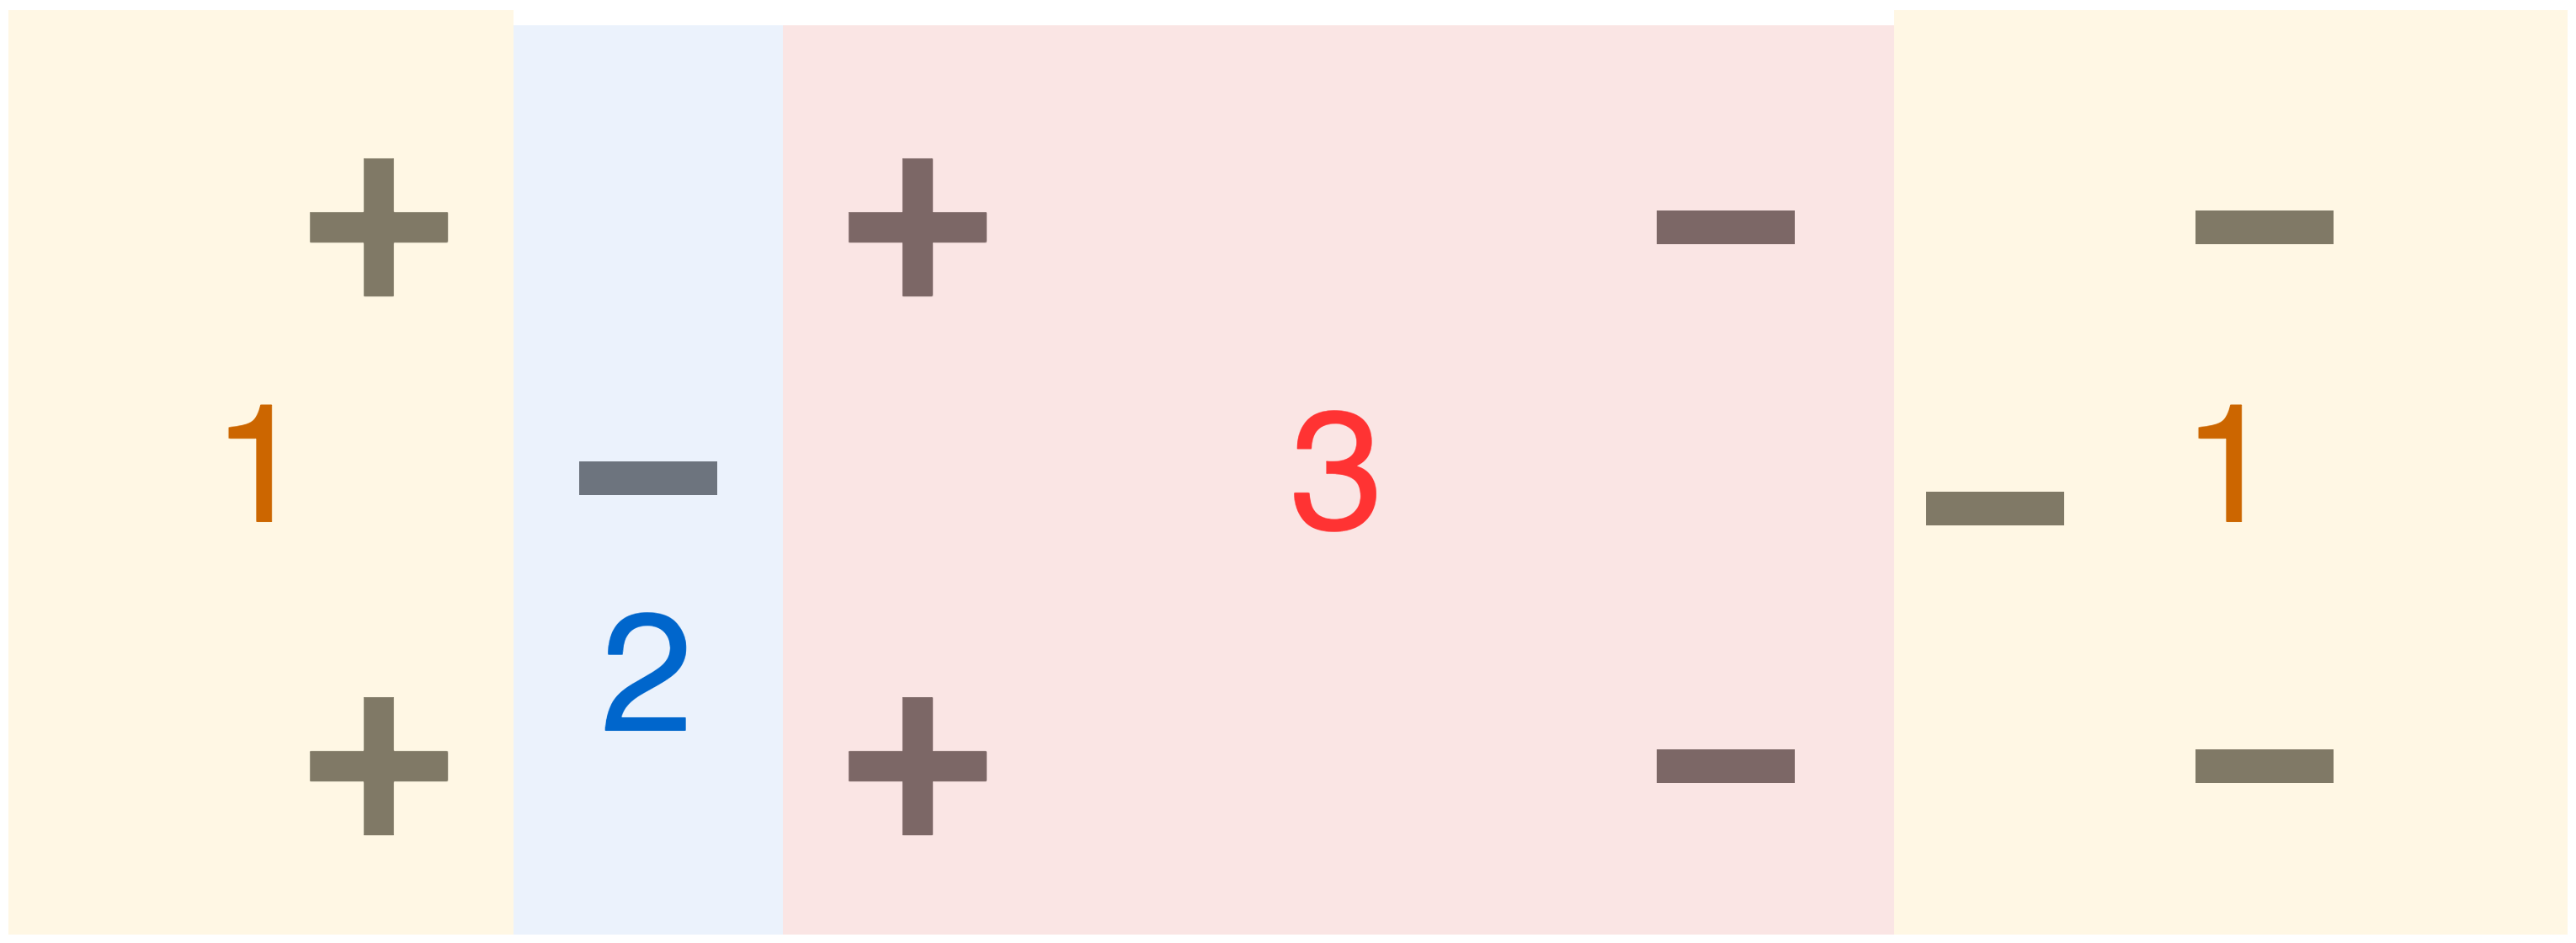
\includegraphics[scale=0.3]{images/q1/districts.png}
    \caption{تقسیم داده‌ها به سه ناحیه}
    \label{districts-of-samples}
\end{figure}

از آن جا که هدف ما کمینه کردن خطای \lr{LOOCV} است، بنابراین در درجه‌ اول سعی می‌کنیم داده‌های موجود در
ناحیه ۳ به درستی برچسب زده شود. در قدم بعدی سعی می‌کنیم داده‌ی موجود در ناحیه ۲ نیز به درستی برچسب بخورد.
در شکل \ref{distance-of-positive-data-relative-to-others} فاصله‌ی نسبی یکی از داده‌های موجود در ناحیه ۳
از سایر داده‌ها رسم شده است.

\begin{figure}[h]
    \centering
    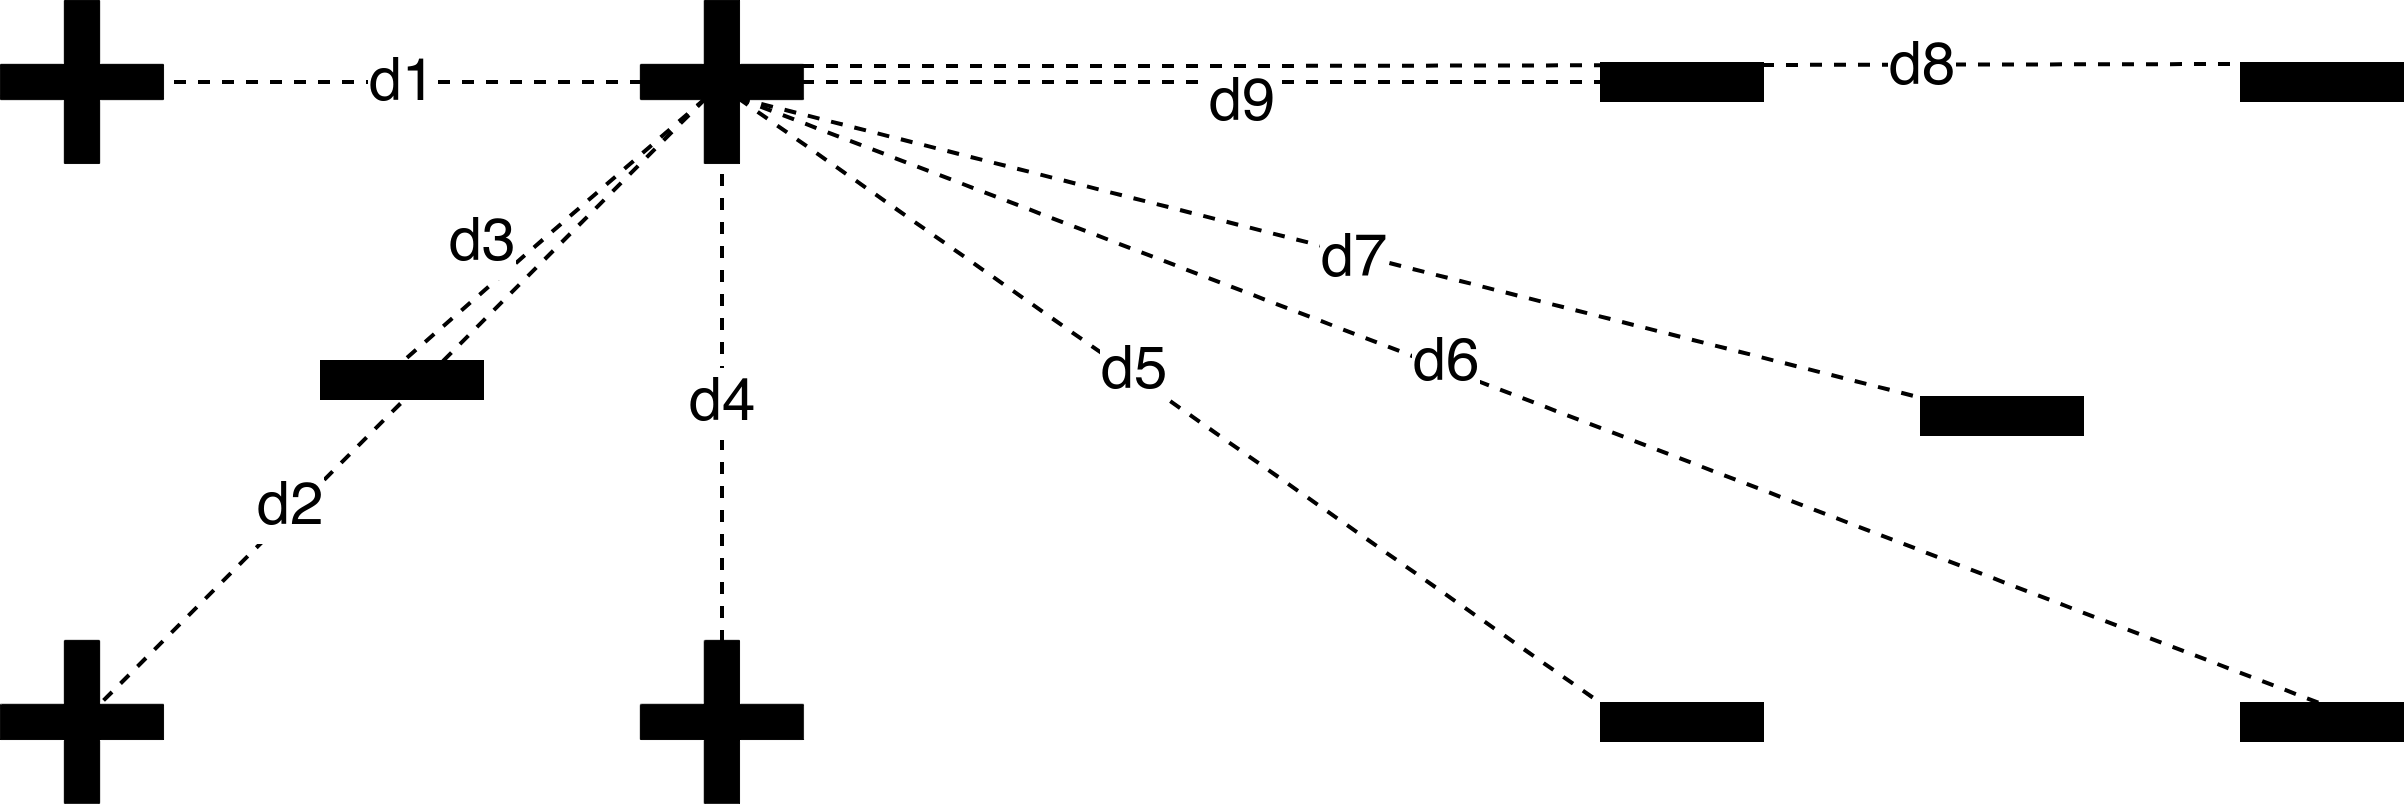
\includegraphics[scale=0.4]{images/q1/distances.png}
    \caption{داده‌ی مثبتی که انتخاب $k$ تاثیر زیادی در نتیجه‌ی آن دارد.}
    \label{distance-of-positive-data-relative-to-others}
\end{figure}

با توجه به شکل رابطه‌‌ی بین $d_i$ها به شکل زیر است. (فواصل مربوط به داده‌های مثبت با رنگ سبز
و فواصل مربوط به داده‌های منفی با رنگ قرمز مشخص شده است.)

$$\textcolor{red}{d_3} < \textcolor{green}{d_1} = \textcolor{green}{d_4} < \textcolor{red}{d_9} <
\textcolor{green}{d_2} < \textcolor{red}{d_5} < \textcolor{red}{d_8} < \textcolor{red}{d_7} < \textcolor{red}{d_6} $$

با توجه به فاصله‌های بالا برای آن‌ که این داده به درستی برچسب زده شود، باید

$$2 < k < 6$$

البته $k=2$ یا $k=6$ نیز به شرطی قابل قبول هستند که به برچسب مثبت اولویت بیشتری داده شود.
بنابراین اگر $2 \leq k \leq 6$ باشد، داده‌های موجود در ناحیه ۳ به درستی برچسب می‌خورد. برای آن که
داده‌ی موجود در ناحیه ۲ به درستی برچسب بخورد حداقل $k$ باید برابر 9 باشد. اما با انتخاب $k=9$
بسیاری از داده‌ها برچسب اشتباه برچسب زده می‌شوند. درنتیجه برای رسیدن به کمترین خطای \lr{LOOCV}
باید از درست‌ برچسب خوردن این داده صرف نظر کنیم، در نتیجه با انتخاب $2 \leq k \leq 6$ به کمترین
خطای \lr{LOOCV} می‌رسیم.

\subsection*{قسمت ب}

بر طبق یک قاعده‌ی سرانگشتی\LTRfootnote{Rule of Thumb} اگر تعداد $n$ داده آموزشی داشته باشیم، در این صورت
$\sqrt{n}$ یک مقدار خوب برای $k$ است. اما در حالت کلی روش عملی برای پیدا کردن مقدار بهینه $k$ وجود ندارد.
معمولا برای پیدا کردن مقدار بهینه $k$، مقادیر مختلفی را برای $k$ در نظر گرفته و با تکرار روش \lr{k-Fold Cross Validation}
مقداری از $k$ که به ازای آن خطای کمینه می‌شود را انتخاب می‌کنند.

\section*{سوال دو}

الگوریتم درخت تصمیم‌گیر نسبت به الگوریتم \lr{KNN} مولدتر\LTRfootnote{Generative} است. برای مثال درخت تصمیمی
را که در شکل \ref{decision-tree-example} آورده شده است در نظر بگیرید. این درخت خانه‌هایی را که ارزش خرید
بالایی دارند را تفکیک می‌کند. با توجه به شکل و بدون دانستن داده‌هایی که درخت بر اساس آن‌ها دسته‌بندی را انجام داده
است، می‌توان خانه‌های جدیدی را که ارزش خرید بالایی دارند را تولید کرد.

\begin{figure}[h]
    \centering
    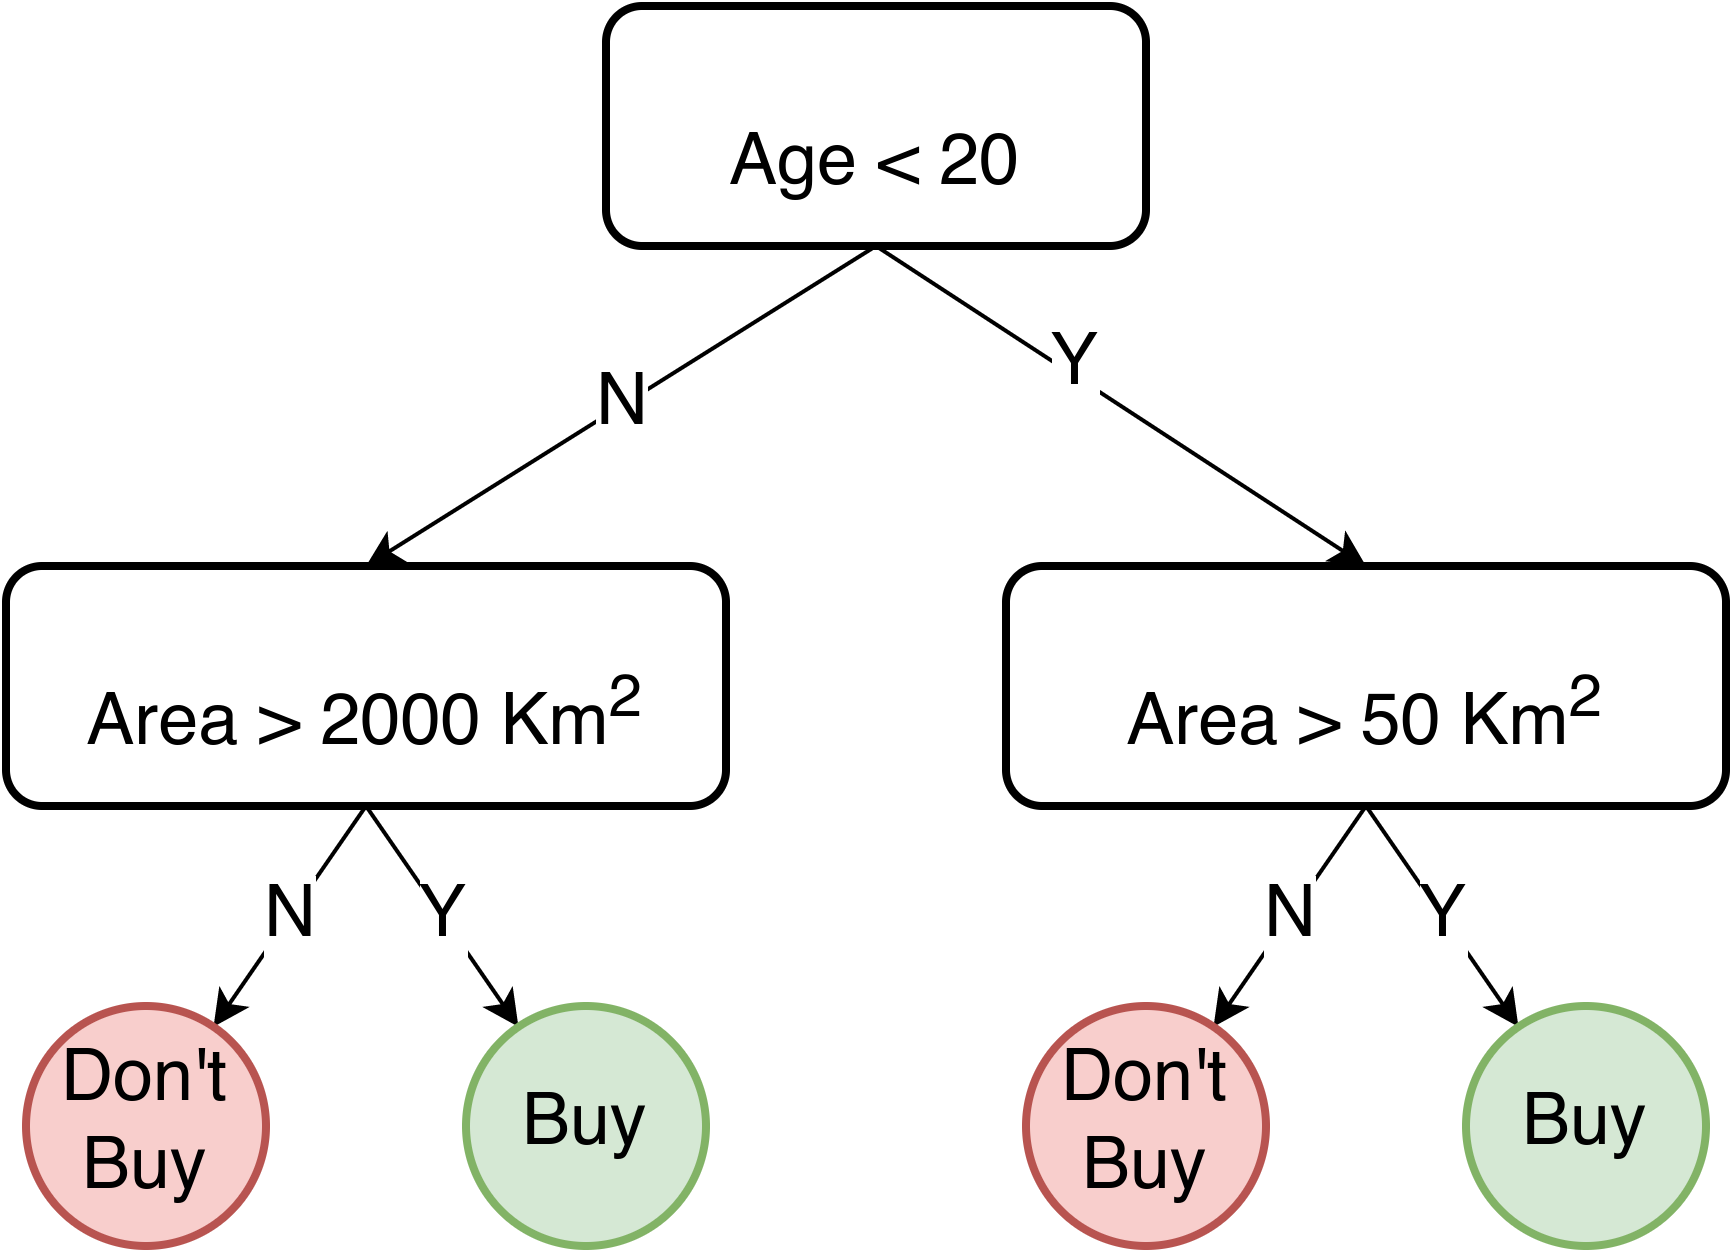
\includegraphics[scale=0.4]{images/q2/decision-tree.png}
    \caption{نمونه‌ای از درخت تصمیم‌گیر}
    \label{decision-tree-example}
\end{figure}

اما همان‌طور که اشاره کردیم، الگوریتم \lr{KNN} یک الگوریتم \lr{Discriminative} است. برای نشان دادن این مطلب
از مثال قبلی کمک می‌گیریم. فرض کنیم درخت تصمیم بر اساس داده‌های موجود در شکل \ref{sample} ساخته شده باشد.
حال همین داده‌ها را به الگوریتم \lr{KNN} داده و از او می‌خواهیم که برچسب نقطه سیاه‌رنگ موجود در شکل را برچسب‌گذاری
کند. این الگوریتم با مقایسه‌ی این داده با داده‌های دیگر می‌تواند این داده را به درستی برچسب بزند، اما نمی‌تواند
داده‌های جدیدی که متعلق به یکی از کلاس‌ها است را بدون مقایسه کردن داده جدید با داده‌های قبلی به دست آورد.

\begin{figure}[h]
    \centering
    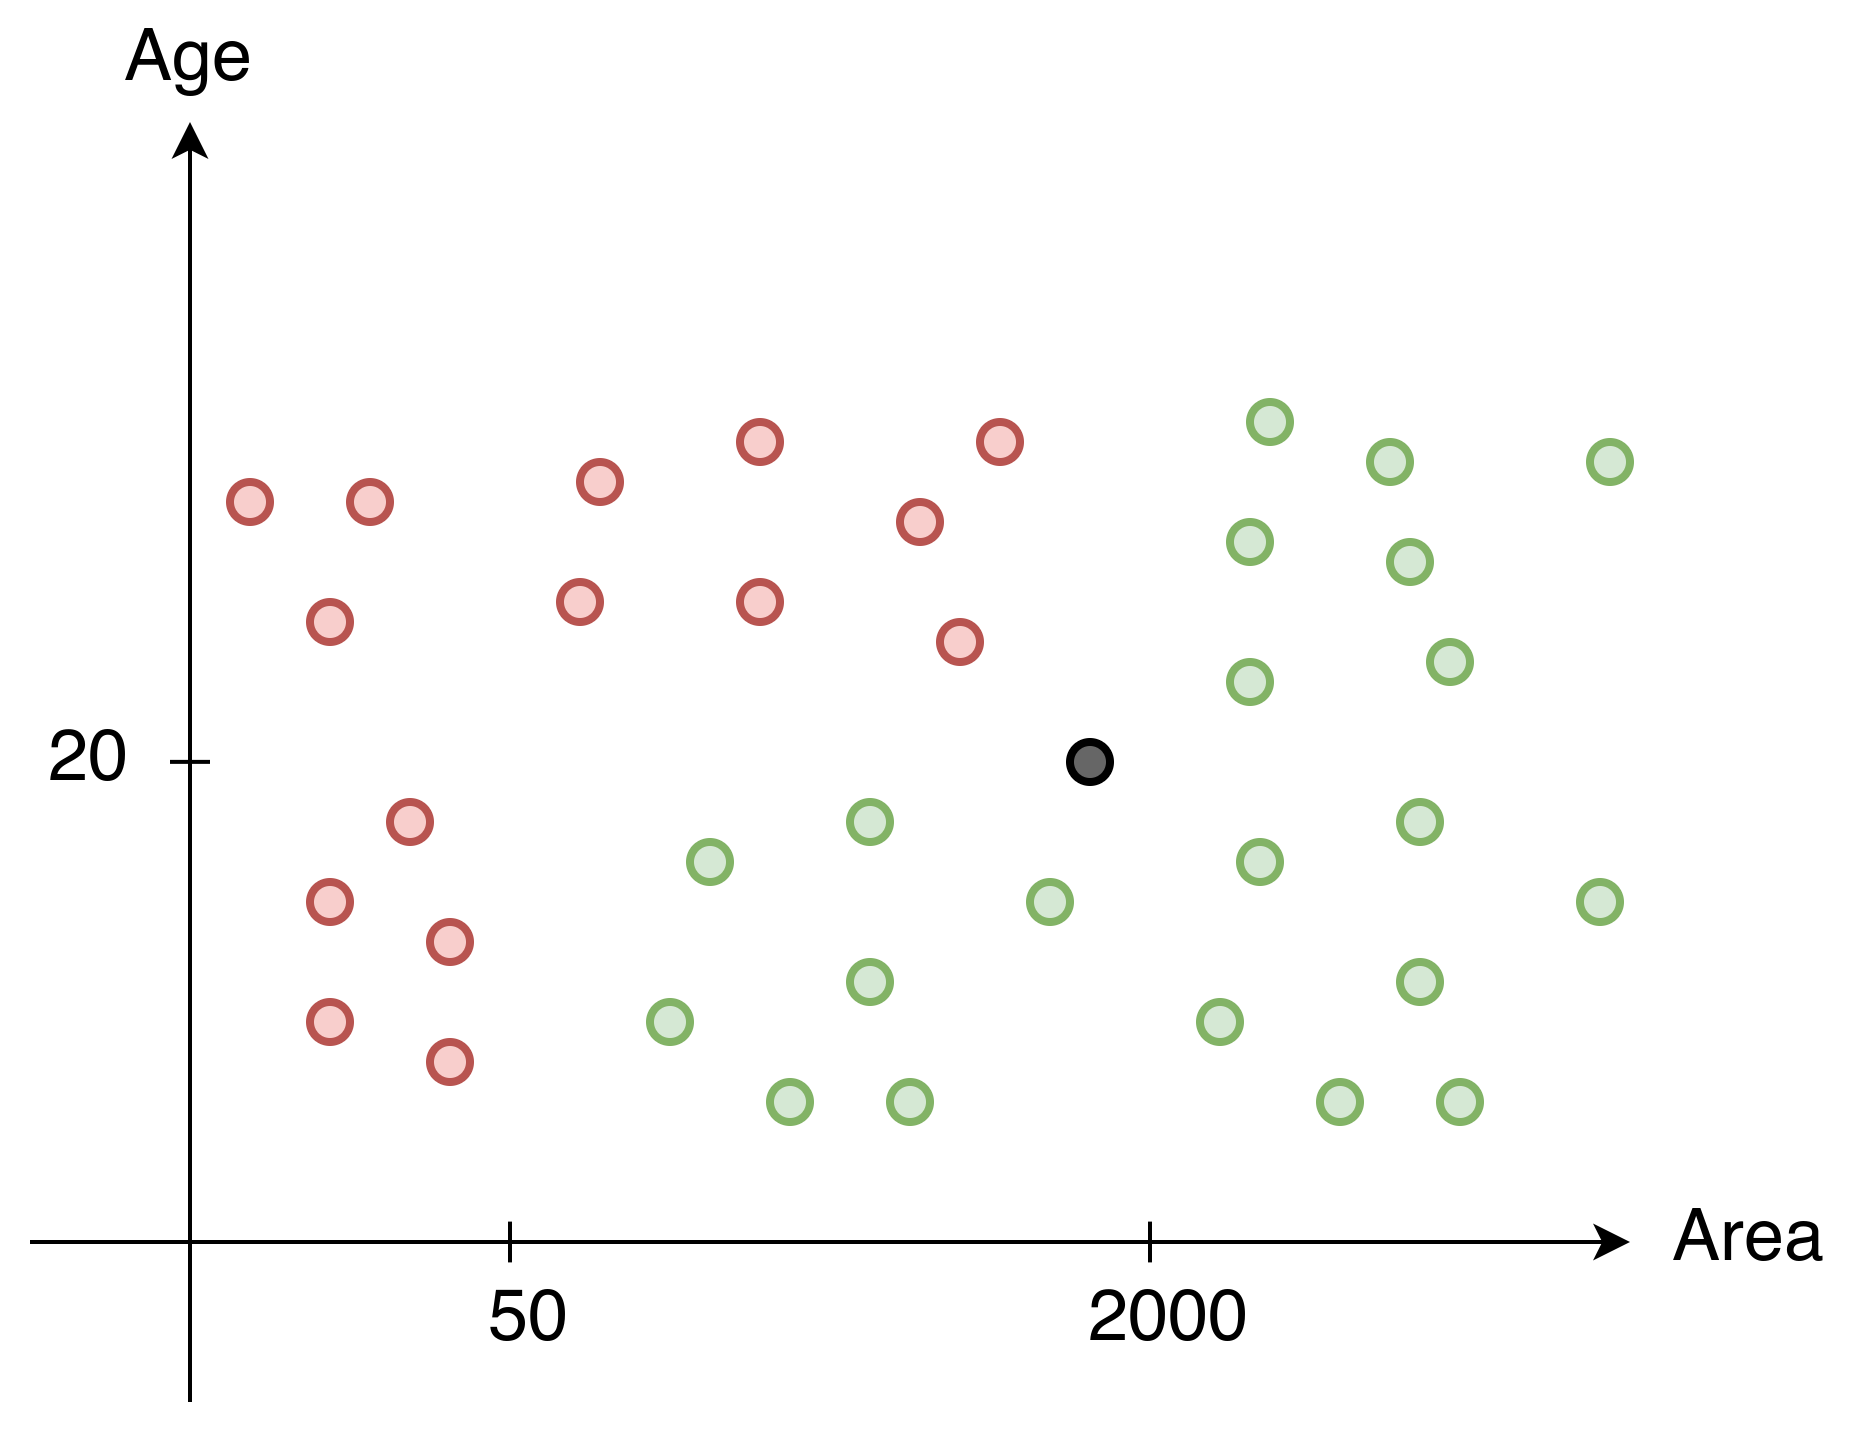
\includegraphics[scale=0.4]{images/q2/samples.png}
    \caption{داده‌های آموزشی به همراه داده‌ی برچسب نخورده}
    \label{sample}
\end{figure}

\section*{سوال سه}

\subsection*{قسمت الف}

داریم.

$$\sigma(a) = \frac{1}{1+e^{-a}}$$

بنابراین.

\begin{eqnarray*}
    \frac{d\sigma(a)}{da} = \frac{0-(-1)e^{-a}}{(1+e^{-a})^2} & = & \frac{e^{-a}}{(1+e^{-a})^2} \\
    & = & \frac{1}{1+e^{-a}} \times \frac{e^{-a}}{1+e^{-a}} \\
    & = & \frac{1}{1+e^{-a}} \times (1 - \frac{1}{1+e^{-a}}) \\
    & = & \sigma(a) (1-\sigma(a)) \\
\end{eqnarray*}

\section*{سوال چهار}

\subsection*{قسمت الف}

با توجه به محاسبات زیر فرد \lr{X1} جنس مد نظر را خریداری می‌کند.

\begin{eqnarray*}
    P(\text{\lr{buy}}=\text{\lr{Yes}}) = \frac{9}{14} & \hspace{2cm} & P(\text{\lr{buy}}=\text{\lr{No}}) = \frac{5}{14}\\
    P(\text{\lr{age}}=\text{\lr{Youth}}) = \frac{2}{9} & \hspace{2cm} & P(\text{\lr{age}}=\text{\lr{Youth}}) = \frac{3}{5}\\
    P(\text{\lr{income}}=\text{\lr{High}}) = \frac{2}{9} & \hspace{2cm} & P(\text{\lr{income}}=\text{\lr{High}}) = \frac{2}{5}\\
    P(\text{\lr{student}}=\text{\lr{Yes}}) = \frac{6}{9} & \hspace{2cm} & P(\text{\lr{student}}=\text{\lr{Yes}}) = \frac{1}{5}\\
    P(\text{\lr{credit}}=\text{\lr{Fair}}) = \frac{6}{9} & \hspace{2cm} & P(\text{\lr{credit}}=\text{\lr{Fair}}) = \frac{2}{5}\\
\end{eqnarray*}

بنابراین

\begin{eqnarray*}
    P(\text{\lr{buy}}=\text{\lr{Yes}})\prod_{i} P(x_i|\text{\lr{buy}}=\text{\lr{Yes}}) & = &  \frac{9}{14} \times \frac{2}{9} \times \frac{2}{9} \times \frac{6}{9} \times \frac{6}{9} =  \frac{1296}{91854} \simeq 0.014\\
    P(\text{\lr{buy}}=\text{\lr{No}})\prod_{i} P(x_i|\text{\lr{buy}}=\text{\lr{No}})  & = & \frac{5}{14} \times \frac{3}{5} \times \frac{2}{5} \times \frac{1}{5} \times \frac{2}{5} = \frac{60}{8750} \simeq 0.006
\end{eqnarray*}

\begin{center}
\rule{0.5\linewidth}{0.1pt}
\end{center}

با توجه به محاسبات زیر فرد \lr{X2} جنس مورد نظر را خریداری نمی‌کند.

\begin{eqnarray*}
    P(\text{\lr{buy}}=\text{\lr{Yes}}) = \frac{9}{14} & \hspace{2cm} & P(\text{\lr{buy}}=\text{\lr{No}}) = \frac{5}{14}\\
    P(\text{\lr{age}}=\text{\lr{Senior}}) = \frac{3}{9} & \hspace{2cm} & P(\text{\lr{age}}=\text{\lr{Senior}}) = \frac{2}{5}\\
    P(\text{\lr{income}}=\text{\lr{Low}}) = \frac{3}{9} & \hspace{2cm} & P(\text{\lr{income}}=\text{\lr{Low}}) = \frac{1}{5}\\
    P(\text{\lr{student}}=\text{\lr{No}}) = \frac{3}{9} & \hspace{2cm} & P(\text{\lr{student}}=\text{\lr{No}}) = \frac{4}{5}\\
    P(\text{\lr{credit}}=\text{\lr{Excellent}}) = \frac{3}{9} & \hspace{2cm} & P(\text{\lr{credit}}=\text{\lr{Excellent}}) = \frac{3}{5}\\
\end{eqnarray*}

بنابراین

\begin{eqnarray*}
    P(\text{\lr{buy}}=\text{\lr{Yes}})\prod_{i} P(x_i|\text{\lr{buy}}=\text{\lr{Yes}}) & = &  \frac{9}{14} \times \frac{3}{9} \times \frac{3}{9} \times \frac{3}{9} \times \frac{3}{9} =  \frac{324}{91854} \simeq 0.007\\
    P(\text{\lr{buy}}=\text{\lr{No}})\prod_{i} P(x_i|\text{\lr{buy}}=\text{\lr{No}})  & = & \frac{5}{14} \times \frac{2}{5} \times \frac{1}{5} \times \frac{4}{5} \times \frac{3}{5} = \frac{120}{8750} \simeq 0.013
\end{eqnarray*}

\begin{center}
\rule{0.5\linewidth}{0.1pt}
\end{center}

با توجه به محاسبات زیر فرد \lr{X3} جنس مورد نظر را خریداری می‌کند.

\begin{eqnarray*}
    P(\text{\lr{buy}}=\text{\lr{Yes}}) = \frac{9}{14} & \hspace{2cm} & P(\text{\lr{buy}}=\text{\lr{No}}) = \frac{5}{14}\\
    P(\text{\lr{age}}=\text{\lr{Middle}}) = \frac{4}{9} & \hspace{2cm} & P(\text{\lr{age}}=\text{\lr{Middle}}) = 0 \\
    P(\text{\lr{income}}=\text{\lr{Medium}}) = \frac{4}{9} & \hspace{2cm} & P(\text{\lr{income}}=\text{\lr{Medium}}) = \frac{2}{5}\\
    P(\text{\lr{student}}=\text{\lr{No}}) = \frac{3}{9} & \hspace{2cm} & P(\text{\lr{student}}=\text{\lr{No}}) = \frac{4}{5}\\
    P(\text{\lr{credit}}=\text{\lr{Fair}}) = \frac{6}{9} & \hspace{2cm} & P(\text{\lr{credit}}=\text{\lr{Fair}}) = \frac{2}{5}\\
\end{eqnarray*}

بنابراین

\begin{eqnarray*}
    P(\text{\lr{buy}}=\text{\lr{Yes}})\prod_{i} P(x_i|\text{\lr{buy}}=\text{\lr{Yes}}) & = &  \frac{9}{14} \times \frac{4}{9} \times \frac{4}{9} \times \frac{3}{9} \times \frac{6}{9} = \frac{2592}{91854} \simeq 0.028\\
    P(\text{\lr{buy}}=\text{\lr{No}})\prod_{i} P(x_i|\text{\lr{buy}}=\text{\lr{No}})  & = & \frac{5}{14} \times 0 \times \frac{2}{5} \times \frac{4}{5} \times \frac{2}{5} = 0
\end{eqnarray*}

\subsection*{قسمت ب}

ابتدا متغیری که بیشتری بهره یادگیری را دارد محاسبه کرده و در ریشه قرار می‌دهیم.

\begin{eqnarray*}
    E(S) & = & -(p_{+} \log_2(p_{+}) + p_{-} \log_2(p_{-})) \\
    & = & - (\frac{9}{14} \log_2{\frac{9}{14}} + \frac{5}{14} \log_2(\frac{5}{14})) \\
    & = & 0.819
\end{eqnarray*}
\begin{eqnarray*}
    IG(\text{\lr{Age}}) & = & E(S) - \sum_{v \in {\text{\lr{Youth, Middle, Senior}}}} \frac{|S_v|}{S} E(S_v) \\
    & = & 0.819 - (\frac{5}{14} E(S_{\text{\lr{Youth}}}) + \frac{4}{14} E(S_{\text{\lr{Middle}}}) + \frac{5}{14} E(S_{\text{\lr{Senior}}}))\\
    & \Longrightarrow & E(S_{\text{\lr{Youth}}}) = -(\frac{3}{5} \log_2(\frac{3}{5}) + \frac{2}{5} \log_2(\frac{2}{5})) = 0.970 \\
    & \Longrightarrow & E(S_{\text{\lr{Middle}}}) = -(\frac{0}{4} \log_2(\frac{0}{4}) + \frac{4}{4} \log_2(\frac{4}{4})) = 0 \\
    & \Longrightarrow & E(S_{\text{\lr{Senior}}}) = -(\frac{2}{5} \log_2(\frac{2}{5}) + \frac{3}{5} \log_2(\frac{3}{5})) = 0.970 \\
    & = & 0.819 - (\frac{5}{14} \times 0.970 + \frac{4}{14} \times 0 + \frac{5}{14} \times 0.970) \\
    IG(\text{\lr{Age}}) & = & 0.127
\end{eqnarray*}
\begin{eqnarray*}
    IG(\text{\lr{Income}}) & = & E(S) - \sum_{v \in {\text{\lr{Low, Medium, High}}}} \frac{|S_v|}{S} E(S_v) \\
    & = & 0.819 - (\frac{4}{14} E(S_{\text{\lr{Low}}}) + \frac{6}{14} E(S_{\text{\lr{Medium}}}) + \frac{4}{14} E(S_{\text{\lr{High}}}))\\
    & \Longrightarrow & E(S_{\text{\lr{Low}}}) = -(\frac{1}{4} \log_2(\frac{1}{4}) + \frac{3}{4} \log_2(\frac{3}{4})) = 0.811 \\
    & \Longrightarrow & E(S_{\text{\lr{Medium}}}) = -(\frac{2}{6} \log_2(\frac{2}{6}) + \frac{4}{6} \log_2(\frac{4}{6})) = 0.918 \\
    & \Longrightarrow & E(S_{\text{\lr{High}}}) = -(\frac{2}{4} \log_2(\frac{2}{4}) + \frac{2}{4} \log_2(\frac{2}{4})) = 1 \\
    & = & 0.819 - (\frac{4}{14} \times 0.811 + \frac{6}{14} \times 0.918 + \frac{4}{14} \times 1 )\\
    IG(\text{\lr{Income}}) & = & -0.091
\end{eqnarray*}
\begin{eqnarray*}
    IG(\text{\lr{Student}}) & = & E(S) - \sum_{v \in {\text{\lr{No, Yes}}}} \frac{|S_v|}{S} E(S_v) \\
    & = & 0.819 - (\frac{7}{14} E(S_{\text{\lr{No}}}) + \frac{7}{14} E(S_{\text{\lr{Yes}}})))\\
    & \Longrightarrow & E(S_{\text{\lr{No}}}) = -(\frac{4}{7} \log_2(\frac{4}{7}) + \frac{3}{7} \log_2(\frac{3}{7})) = 0.985 \\
    & \Longrightarrow & E(S_{\text{\lr{Yes}}}) = -(\frac{1}{7} \log_2(\frac{1}{7}) + \frac{6}{7} \log_2(\frac{6}{7})) = 0.591 \\
    & = & 0.819 - (\frac{7}{14} \times 0.985 + \frac{7}{14} \times 0.591 )\\
    IG(\text{\lr{Student}}) & = & 0.03
\end{eqnarray*}
\begin{eqnarray*}
    IG(\text{\lr{Credit}}) & = & E(S) - \sum_{v \in {\text{\lr{Fair, Excellent}}}} \frac{|S_v|}{S} E(S_v) \\
    & = & 0.819 - (\frac{8}{14} E(S_{\text{\lr{Fair}}}) + \frac{6}{14} E(S_{\text{\lr{Excellent}}})))\\
    & \Longrightarrow & E(S_{\text{\lr{Fair}}}) = -(\frac{2}{8} \log_2(\frac{2}{8}) + \frac{6}{8} \log_2(\frac{6}{8})) = 0.811 \\
    & \Longrightarrow & E(S_{\text{\lr{Excellent}}}) = -(\frac{3}{6} \log_2(\frac{3}{6}) + \frac{3}{6} \log_2(\frac{3}{6})) = 1 \\
    & = & 0.819 - (\frac{8}{14} \times 0.811 + \frac{6}{14} \times 1 )\\
    IG(\text{\lr{Credit}}) & = & -0.072
\end{eqnarray*}

با توجه به این محاسبات بهترین ویژگی برای ریشه \lr{Age} است. ادامه روال را نیز می‌توان با محاسبه‌
بهره اطلاعاتی پیش رفت، اما برای ساده‌تر شدن، سعی می‌کنیم با بحث روی مقادیر جدول مسئله را حل کنیم.
در حال حاضر درخت ما دارای سه گره است. در ادامه وضعیت جدول به ازای هر یک از این گره‌ها را بررسی می‌کنیم.

\begin{enumerate}
    \item شاخه‌ \lr{Youth}: با انتخاب \lr{Age = Youth} جدول به شکل \ref{youth-branch} در می‌آید. همان‌طور که مشاهده
    می‌شود در این جدول با استفاده از ویژگی \lr{Student} جدول را به دو شاخه کاملا خالص تبدیل کرد در صورتی که
    چنین اتفاقی با انتخاب سایر ویژگی‌ها رخ نمی‌دهد.
    \begin{figure}[h]
        \centering
        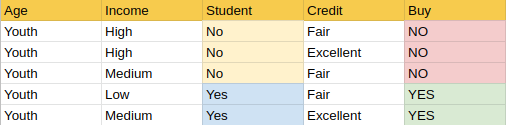
\includegraphics[scale=0.5]{images/q4/youth.png}
        \caption{در گره \lr{Youth} جدول به این شکل در می‌آید.}
        \label{youth-branch}
    \end{figure}
    \item شاخه‌ \lr{Middle}: با توجه به آن که به ازای انتخاب \lr{Age=Middle} به یک شاخه کاملا خالص می‌رسیم،
    بنابراین در این شاخه بحثی برای ادامه دسته‌بندی باقی نمی‌ماند. (شکل \ref{middle-branch})
    \begin{figure}[h]
        \centering
        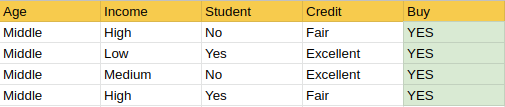
\includegraphics[scale=0.5]{images/q4/middle.png}
        \caption{در گره \lr{Middle} جدول به این شکل در می‌آید.}
        \label{middle-branch}
    \end{figure}
    \item شاخه‌ \lr{Senior}: با انتخاب \lr{Age = Senior} جدول به شکل \ref{senior-branch} در می‌آید. همان‌طور که مشاهده
    می‌شود در این حالت نیز مشابه اتفاقی که در شاخه \lr{Youth} افتاد، رخ می‌دهد.
    \begin{figure}[h]
        \centering
        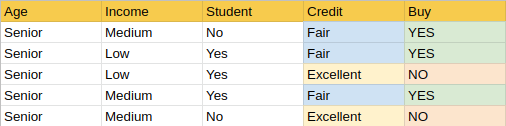
\includegraphics[scale=0.5]{images/q4/senior.png}
        \caption{در گره \lr{Senior} جدول به این شکل در می‌آید.}
        \label{senior-branch}
    \end{figure}
\end{enumerate}

با توجه به توضیحات درخت تصمیم به شکل \ref{q4-final-decision-tree} حاصل می‌شود.

\begin{figure}[h]
    \centering
    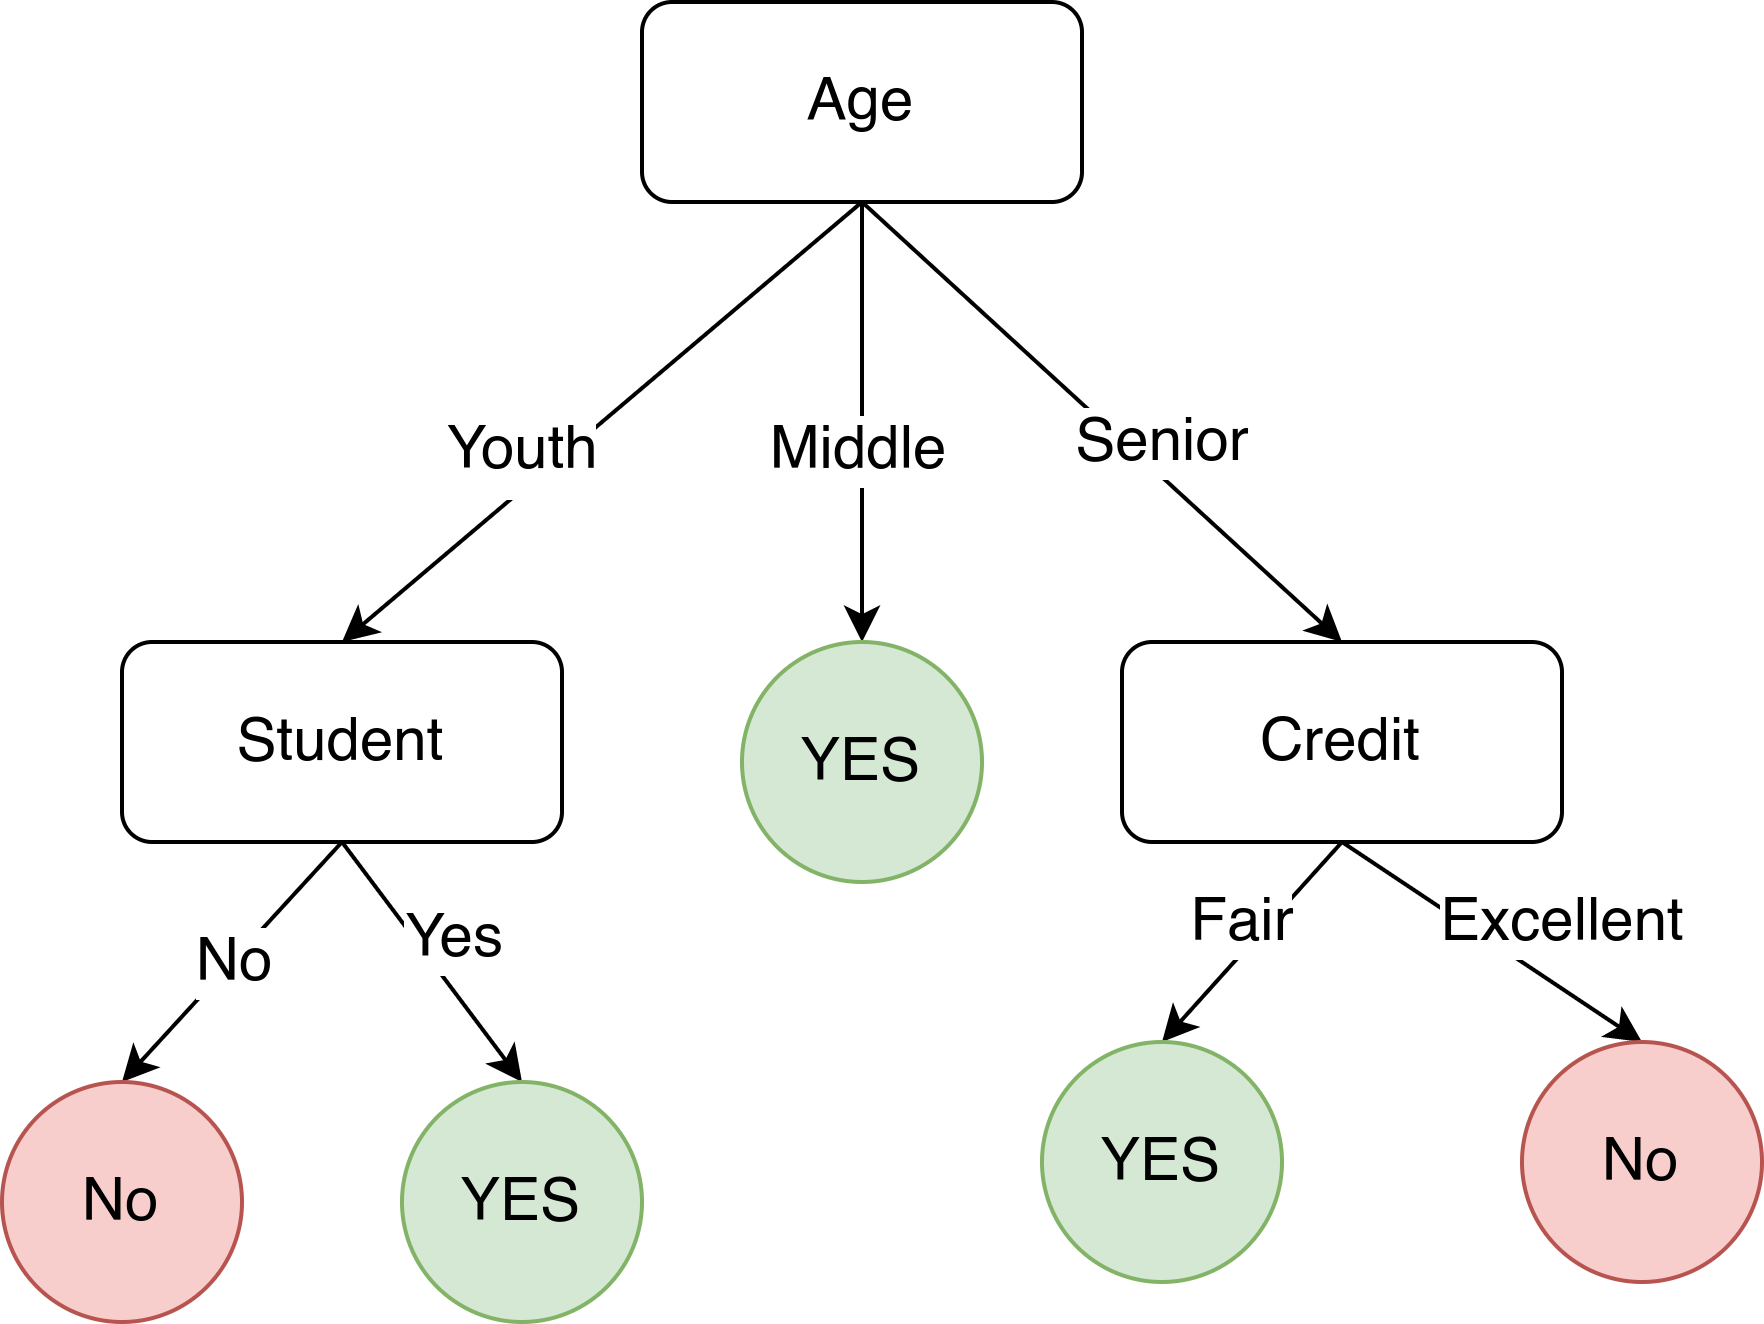
\includegraphics[scale=0.5]{images/q4/decision-tree.png}
    \caption{درخت تصمیم سوال چهار قسمت ب}
    \label{q4-final-decision-tree}
\end{figure}

\section*{سوال پنج}

\subsection*{قسمت الف}

برای انجام دسته‌بندی از الگوریتم \lr{REPTree} استفاده می‌کنیم.
خروجی‌های این کد در شکل \ref{question5-parta} آورده شده است.

\begin{figure}[h]
    \begin{subfigure}{0.48\linewidth}
        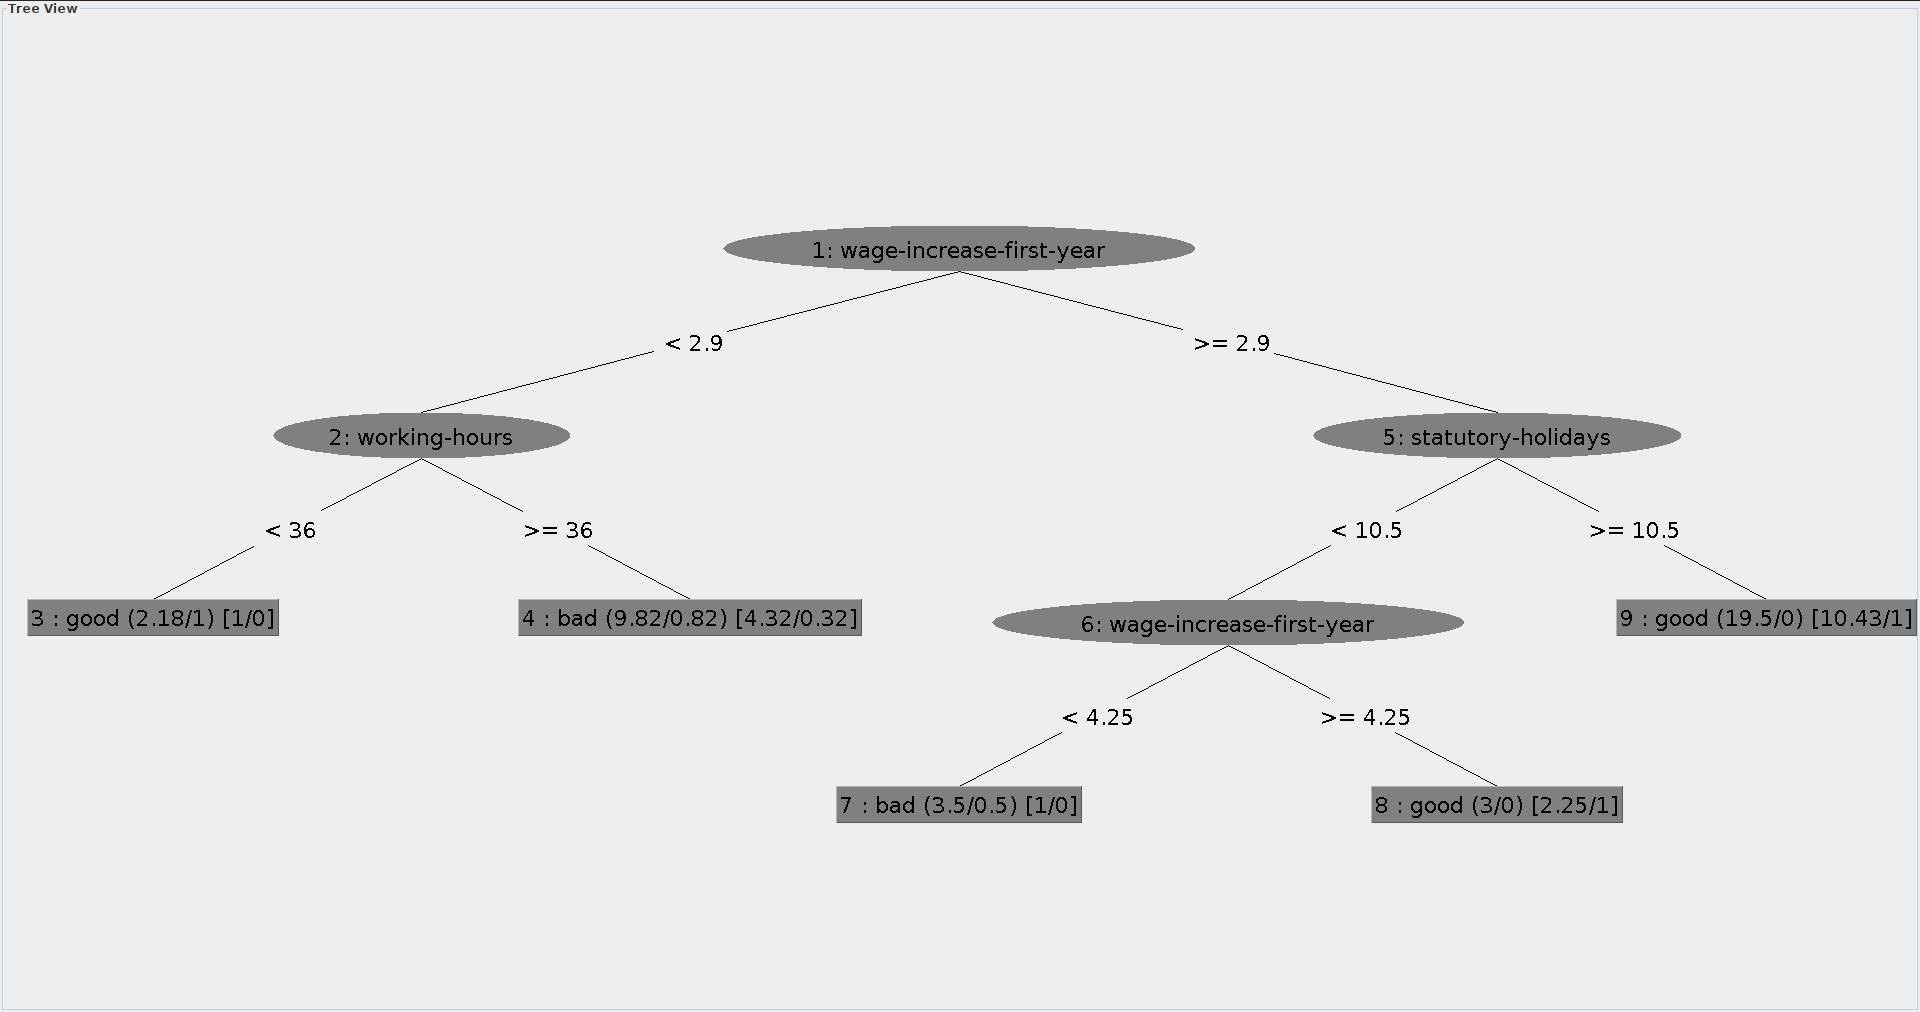
\includegraphics[width=\linewidth]{images/q5/tree_visualization.png}
        \caption{درخت تصمیم‌گیر تولید شده}
    \end{subfigure}
    \hfill
    \begin{subfigure}{0.48\linewidth}
        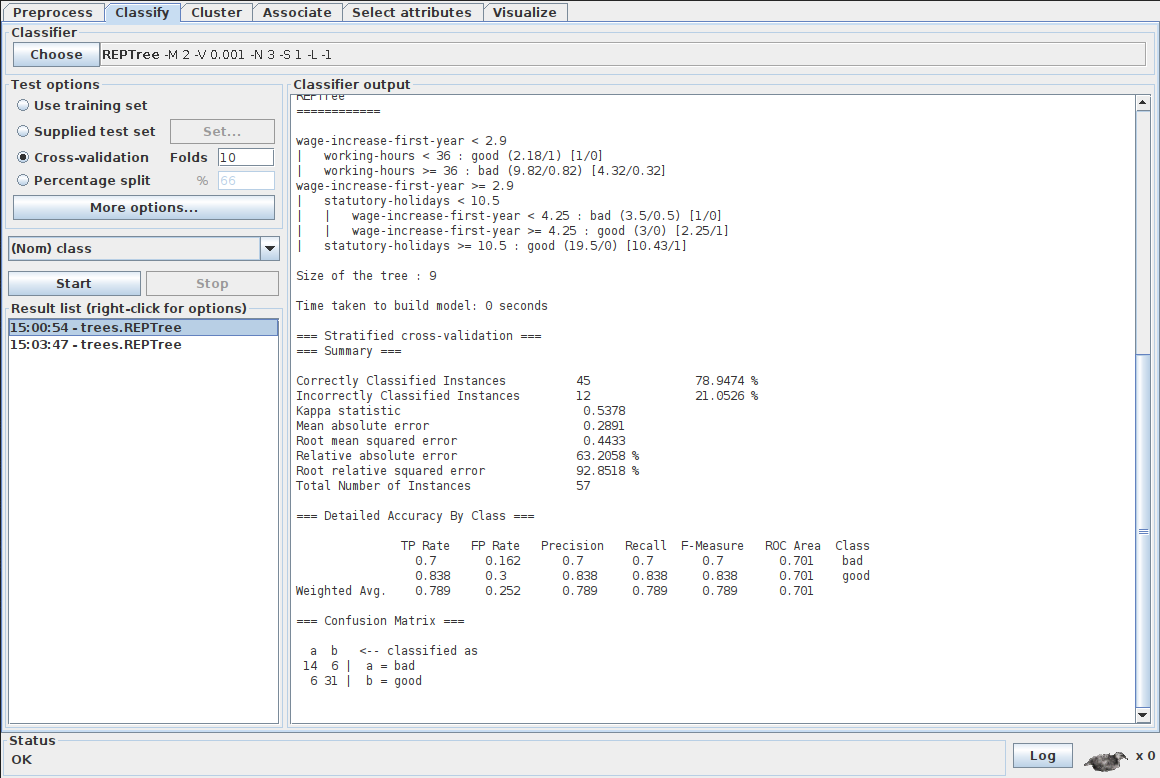
\includegraphics[width=\linewidth]{images/q5/weka_tree_generator.png}
        \caption{پنجره مربوط به درخت تصمیم‌گیر در نرم‌افزار \lr{Weka}}
    \end{subfigure}
    \caption{شکل سوال پنج قسمت الف}
    \label{question5-parta}
\end{figure}

\subsection*{قسمت ب}

در پنجره نرم‌افزار \lr{Weka}ماتریس در هم ریختگی گزارش شده است. تصویر این ماتریس در شکل
\ref{q5-confusion-matrix} آورده شده است.

\begin{figure}[h]
    \centering
    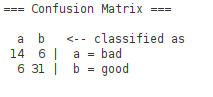
\includegraphics[scale=0.5]{images/q5/confusion_matrix.png}
    \caption{درخت تصمیم سوال پنج قسمت ب}
    \label{q5-confusion-matrix}
\end{figure}

\subsection*{قسمت ج}

درخت تصمیم به صورت موجود در شکل \ref{question5-partc} حاصل می‌شود.

\begin{figure}[h]
    \begin{subfigure}{0.48\linewidth}
        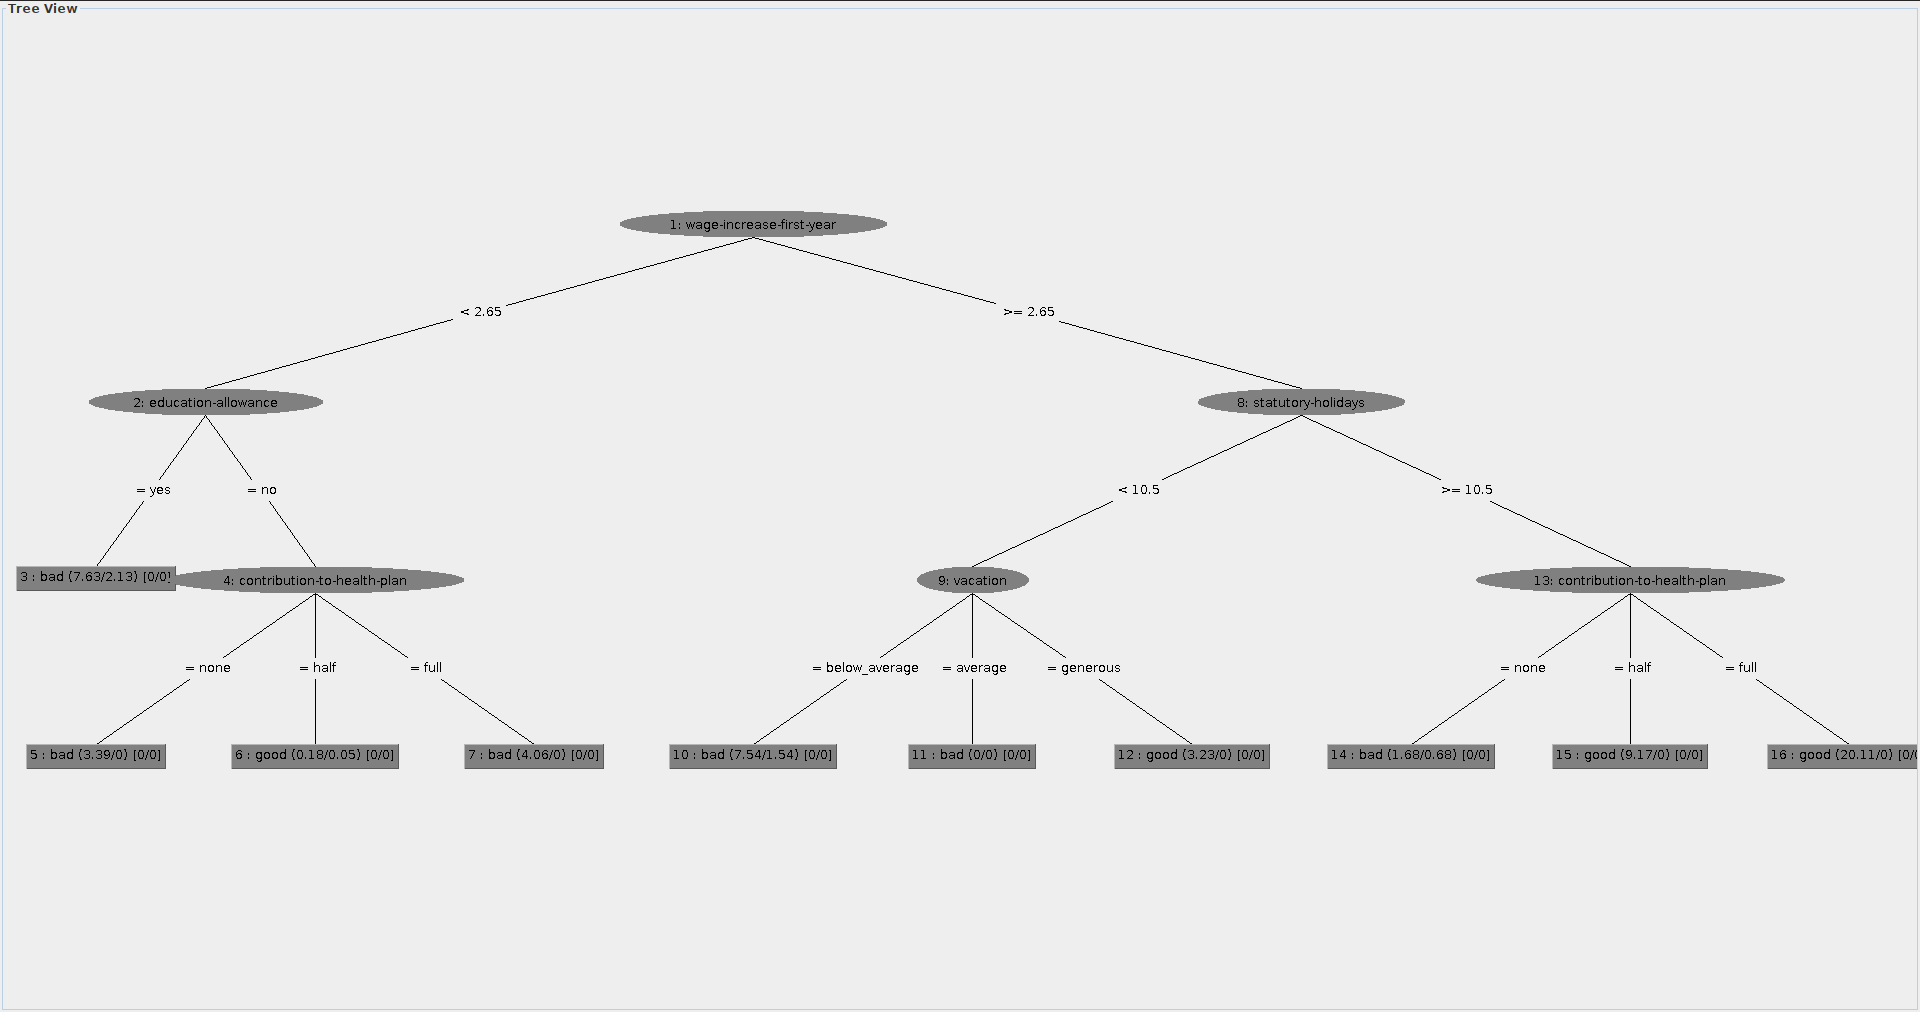
\includegraphics[width=\linewidth]{images/q5/tree_visualization_no_pruning.png}
        \caption{درخت تصمیم‌گیر تولید شده در حالت بدون هرس}
    \end{subfigure}
    \hfill
    \begin{subfigure}{0.48\linewidth}
        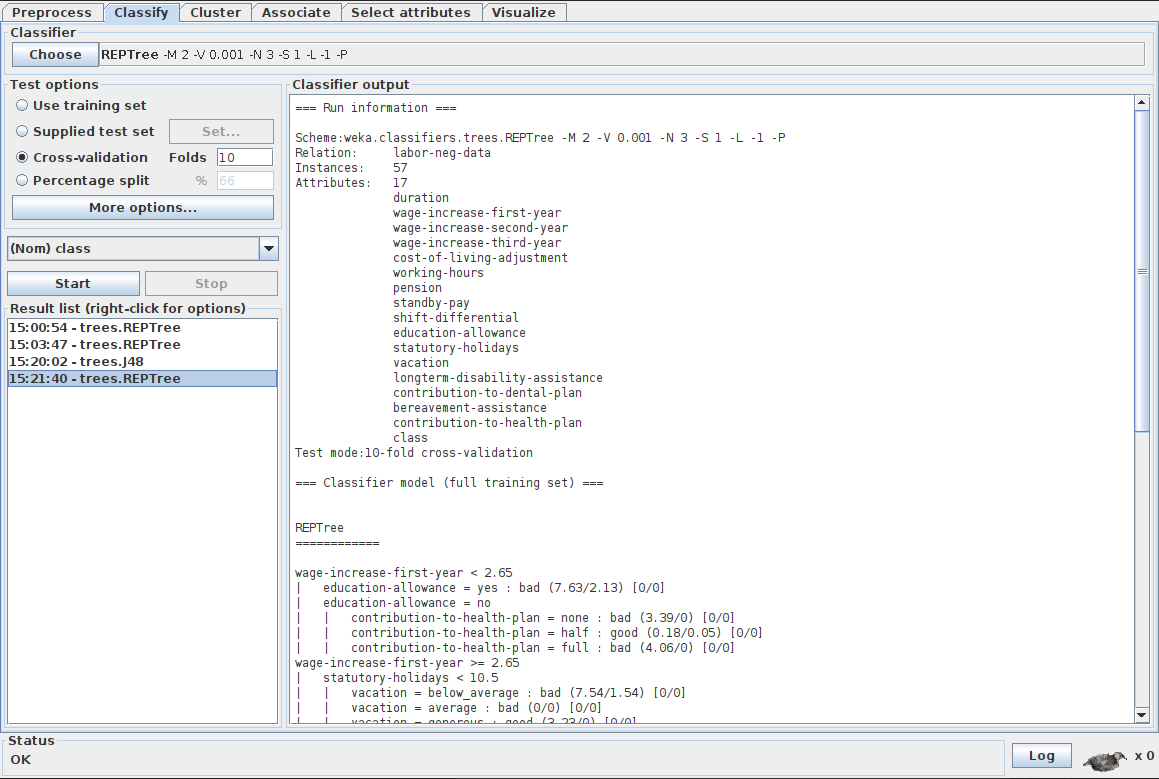
\includegraphics[width=\linewidth]{images/q5/weka_tree_generator_no_pruning.png}
        \caption{پنجره مربوط به درخت تصمیم‌گیر بدون انجام عملیات هرس در نرم‌افزار \lr{Weka}}
    \end{subfigure}
    \caption{شکل سوال پنج قسمت ج}
    \label{question5-partc}
\end{figure}

\subsection*{قسمت د}

همان طور که انتظار می‌رفت هنگامی که درخت هرس نمی‌شود، درخت بزرگ‌تری تولید می‌شود. در حالت هرس کردن
با وجود آن که نتیجه روی داده‌های آموزشی اندکی افت پیدا می‌کند اما درخت تولید شده عملکرد بهتری
روی داده‌های تست دارد. درخت‌های تصمیم مربوط به هر یک از این حالات در شکل \ref{question5-parta}
و \ref{question5-partc} رسم شده است.

\section*{سوال‌های پیاده‌سازی}

\section*{سوال سه}

\subsection*{قسمت الف}

برای یافتن بهترین مقدار $k$ تنها مقادیر فردی را که در بازه $[1,30]$ قرار دارند را بررسی می‌کنیم.
دقت‌های حاصل شده در شکل \ref{implementation-question1-parta} مشاهده می‌شود. همان‌طور که مشاهده می‌شود،
به ازای $k=1$ بهترین دقت حاصل شده است.


\begin{figure}[h]
    \centering
    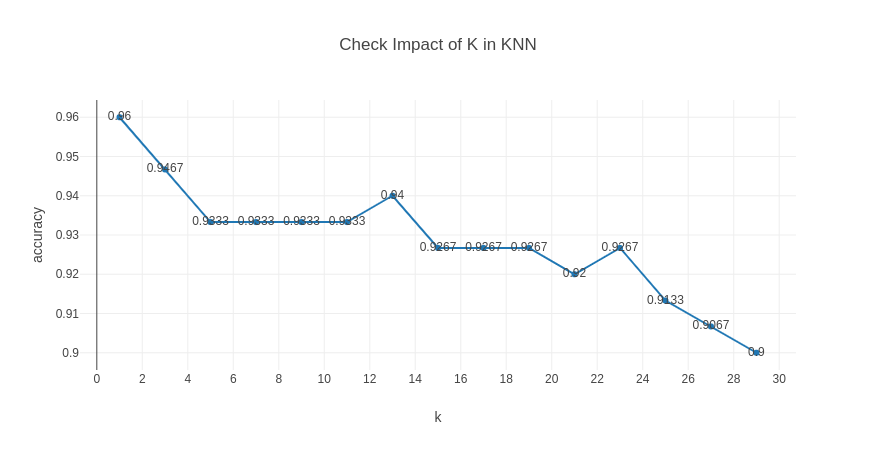
\includegraphics[width=\linewidth]{images/implementation/q1/parta.png}
    \caption{دقت‌های حاصل شده به ازای مقادیر مختلف $k$}
    \label{implementation-question1-parta}
\end{figure}

\subsection*{قسمت ب}

جدول درهم‌ریختگی این دسته‌بند در شکل \ref{implementation-question1-partb} آورده شده است. در این شکل جدول‌های متناظر
داده‌های آموزش و تست نشان داده شده است. با توجه به این جداول دقت در داده‌ی آموزشی
برابر $100$ درصد و در داده‌های تست برابر $96.67$ درصد است.

\begin{figure}[h]
    \begin{subfigure}{0.48\linewidth}
        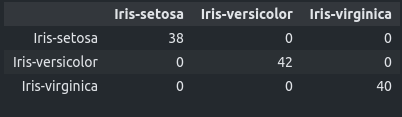
\includegraphics[width=\linewidth]{images/implementation/q1/train_confusion_matrix.png}
        \caption{جدول درهم‌ریختگی داده‌های آموزش}
    \end{subfigure}
    \hfill
    \begin{subfigure}{0.48\linewidth}
        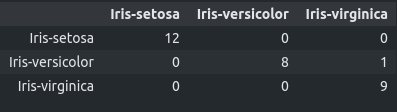
\includegraphics[width=\linewidth]{images/implementation/q1/test_confusion_matrix.png}
        \caption{جدول درهم‌ریختگی داده‌های تست}
    \end{subfigure}
    \caption{شکل سوال پنج قسمت ج}
    \label{implementation-question1-partb}
\end{figure}

\end{document}
